\documentclass[11pt]{article}
\usepackage{theme}
\usepackage{shortcuts}
\usepackage{bm}
\usepackage{subcaption}
\usepackage{graphicx}

\title{Mini-Project (ML for Time Series) - MVA 2023/2024 \\ \Large{\textit{Time warp invariant kSVD:\\ Sparse coding and dictionary learning for time series under time warp}}}

\author{
Manal Akhannouss \email{manal.akhannouss@eleves.enpc.fr} \\
Alexandre Lutt \email{alexandre.lutt@eleves.enpc.fr}
}

\begin{document}
\maketitle

\section{Introduction and contributions}

\cite{main_paper}

\section{Method}

\paragraph{} 

\subsection{Sparse coding}

\paragraph{} 

\subsubsection{Orthogonal Matching Pursuit}

\paragraph{} 

\subsubsection{Time Warp Invariant Orthogonal Matching Pursuit}

\paragraph{} 

\subsection{Dictionnary Learning}

\paragraph{} 

\subsubsection{kSVD}

\paragraph{} 

\subsubsection{Time Warp Invariant kSVD}

\paragraph{} 

\subsection{Evaluation metrics}

\paragraph{} 


\section{Data}

\subsection{BME Dataset}

\paragraph{} 

\subsection{DIGITS Dataset}

\paragraph{} 


\section{Results}

\subsection{BME Dataset}

\paragraph{} 

\subsection{DIGITS Dataset}

\paragraph{} 


\begin{table*}[!ht]
    \centering
        \begin{tabular}{ccc}
            \toprule
            \textbf{Sparsity/Models} & \textbf{kSVD} & \textbf{TWI-kSVD} \\
            \midrule
            \textbf{2} & $0.25551$ & $0.17313$ \\
            \textbf{5} & $0.19873$ & $0.12301$ \\
            \textbf{10} & $\bm{0.15060}$ & $\bm{0.08559}$ \\
            \bottomrule
        \end{tabular}
    \caption{Reconstruction $L_2$ errors on the BME dataset (lower is better)}
    \label{tab:reconstruction_results_BME}
\end{table*}

\begin{table*}[!ht]
    \begin{minipage}{.55\linewidth}
      \centering
        \begin{tabular}{ccc}
            \toprule
            \textbf{Sparsity/Models} & \textbf{kSVD} & \textbf{TWI-kSVD} \\
            \midrule
            \textbf{2} & $\bm{0.22}$ & $0.58$ \\
            \textbf{5} & $0.30$ & $0.58$ \\
            \textbf{10} & $0.45$ & $\bm{0.47}$ \\
            \bottomrule
        \end{tabular}
        \caption{Original classification strategy}
    \end{minipage}
    \begin{minipage}{.35\linewidth}
      \centering
        \begin{tabular}{ccc}
            \toprule
            \textbf{Sparsity/Models} & \textbf{kSVD} & \textbf{TWI-kSVD} \\
            \midrule
            \textbf{2} & $\bm{0.07}$ & $\bm{0.53}$ \\
            \textbf{5} & $0.08$ & $\bm{0.53}$ \\
            \textbf{10} & $0.10$ & $0.62$ \\
            \bottomrule
        \end{tabular}
        \caption{Our classification strategy}
    \end{minipage} 
    \caption{Classification error rates on the BME dataset (lower is better)}
    \label{tab:classif_results_BME}
\end{table*}

\begin{table*}[!ht]
    \centering
        \begin{tabular}{ccc}
            \toprule
            \textbf{Sparsity/Models} & \textbf{kSVD} & \textbf{TWI-kSVD} \\
            \midrule
            \textbf{2} & $0.50133$ & $0.53786$ \\
            \textbf{5} & $0.30436$ & $0.32883$ \\
            \textbf{10} & $\bm{0.20911}$ & $\bm{0.21764}$ \\
            \bottomrule
        \end{tabular}
    \caption{Reconstruction $L_2$ errors on the DIGITS dataset (lower is better)}
    \label{tab:reconstruction_results_DIGITS}
\end{table*}

\begin{table*}[!ht]
    \begin{minipage}{.55\linewidth}
      \centering
        \begin{tabular}{ccc}
            \toprule
            \textbf{Sparsity/Models} & \textbf{kSVD} & \textbf{TWI-kSVD} \\
            \midrule
            \textbf{2} & $\bm{0.27}$ & $0.73$ \\
            \textbf{5} & $0.53$ & $\bm{0.66}$ \\
            \textbf{10} & $0.63$ & $0.92$ \\
            \bottomrule
        \end{tabular}
        \caption{Original classification strategy}
    \end{minipage}
    \begin{minipage}{.35\linewidth}
      \centering
        \begin{tabular}{ccc}
            \toprule
            \textbf{Sparsity/Models} & \textbf{kSVD} & \textbf{TWI-kSVD} \\
            \midrule
            \textbf{2} & $\bm{0.14}$ & $0.81$ \\
            \textbf{5} & $0.27$ & $\bm{0.76}$ \\
            \textbf{10} & $0.29$ & $0.88$ \\
            \bottomrule
        \end{tabular}
        \caption{Our classification strategy}
    \end{minipage} 
    \caption{Classification error rates on the DIGITS dataset (lower is better)}
    \label{tab:classif_results_DIGITS}
\end{table*}

\begin{figure*}[!ht]
    \centering
    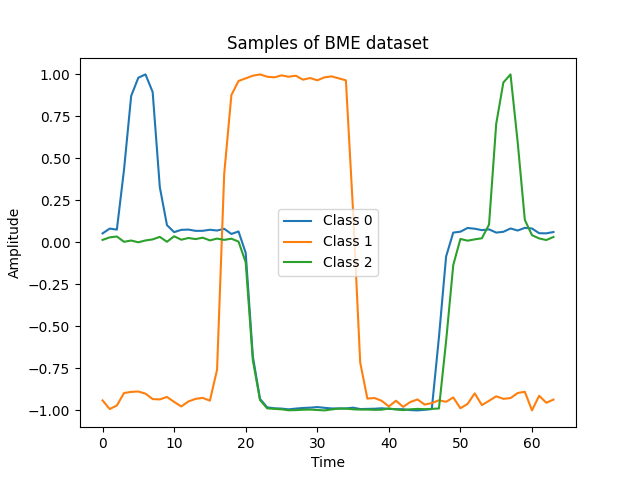
\includegraphics[scale=0.7]{../../figures/BME_samples.png}
    \caption{Samples of each class of the BME dataset} \label{fig:BME_samples}
\end{figure*}


\begin{figure*}[!ht]
    \centering
    \begin{subfigure}[b]{0.49\textwidth}
      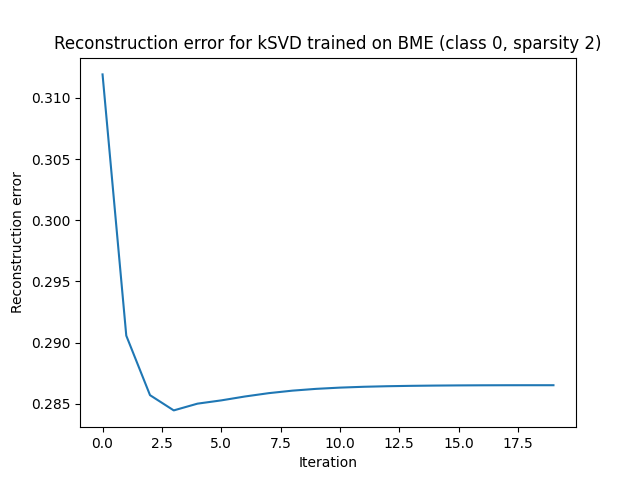
\includegraphics[width=\textwidth]{../../figures/loss_kSVD_spars_2_class_0_BME.png}
      \caption{kSVD}
    \end{subfigure}
    \begin{subfigure}[b]{0.49\textwidth}
        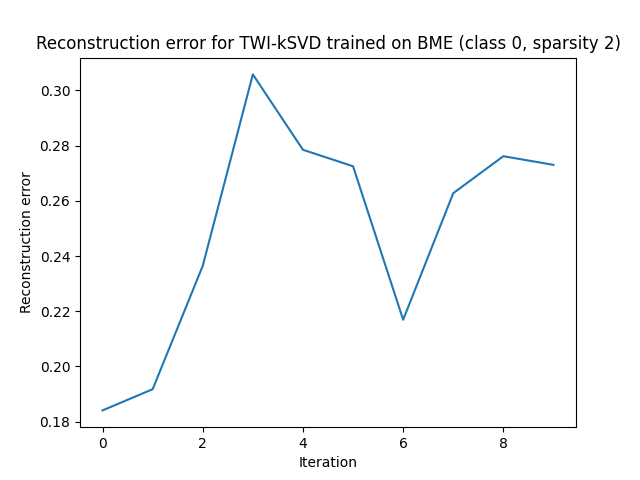
\includegraphics[width=\textwidth]{../../figures/loss_TWI_kSVD_spars_2_class_0_BME.png}
        \caption{TWI-kSVD}
      \end{subfigure}
    \caption{Evolution of reconstruction loss during training (BME dataset)}\label{fig:loss_BME}
\end{figure*}


\begin{figure*}[!ht]
    \begin{subfigure}[b]{0.33\textwidth}
        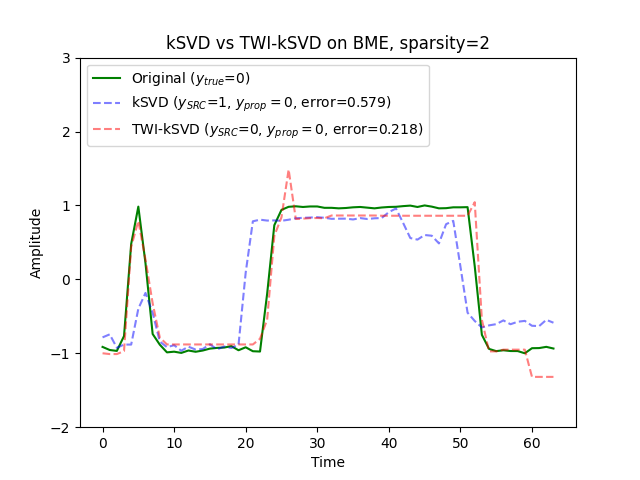
\includegraphics[width=\textwidth]{../../figures/1D_example_sparsity_2.png}
        \caption{Sparsity = 2}
    \end{subfigure}
    \begin{subfigure}[b]{0.33\textwidth}
        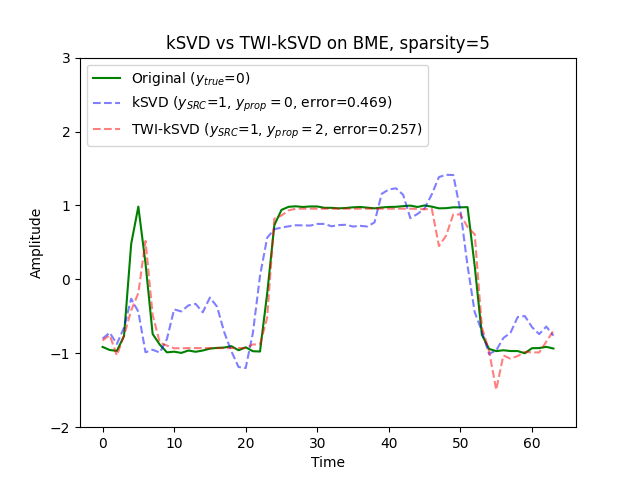
\includegraphics[width=\textwidth]{../../figures/1D_example_sparsity_5.png}
        \caption{Sparsity = 5}
    \end{subfigure}
    \begin{subfigure}[b]{0.33\textwidth}
        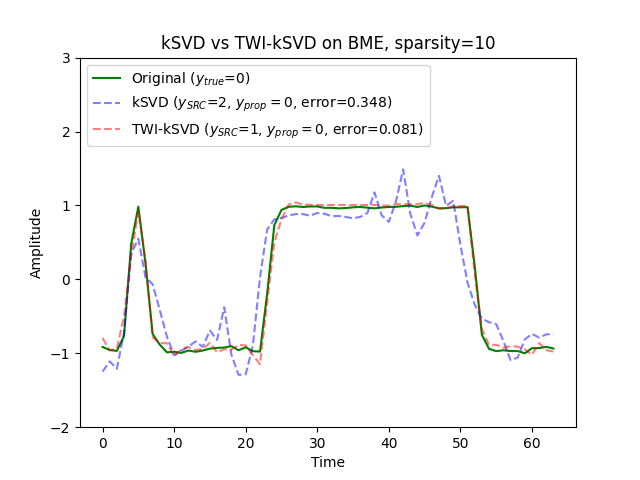
\includegraphics[width=\textwidth]{../../figures/1D_example_sparsity_10.png}
        \caption{Sparsity = 10}
    \end{subfigure}
    \caption{Example of reconstructions (BME dataset) with different sparsity levels}\label{tab:1D_example}
\end{figure*}


\begin{figure*}[!ht]
    \centering
    \begin{subfigure}[t]{\textwidth}
        \centering
        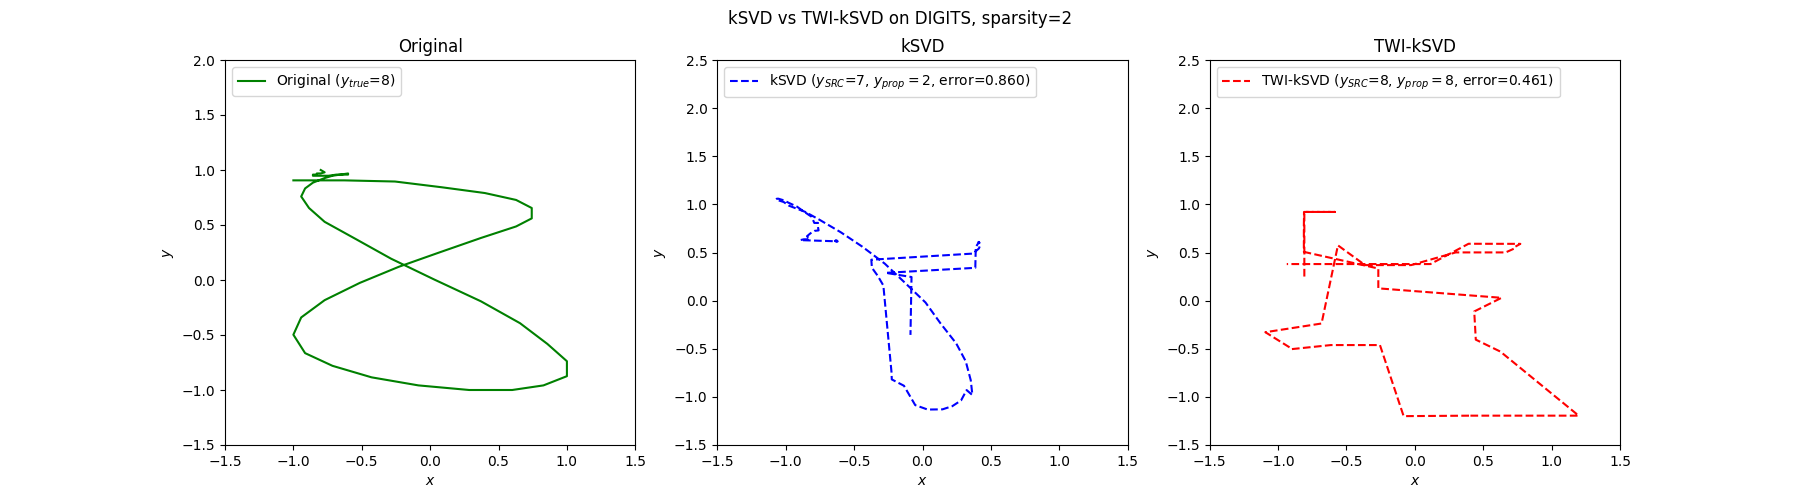
\includegraphics[width=\textwidth]{../../figures/2D_example_sparsity_2.png}
        \caption{Sparsity = 2}
    \end{subfigure}
    
    \begin{subfigure}[t]{\textwidth}
        \centering
        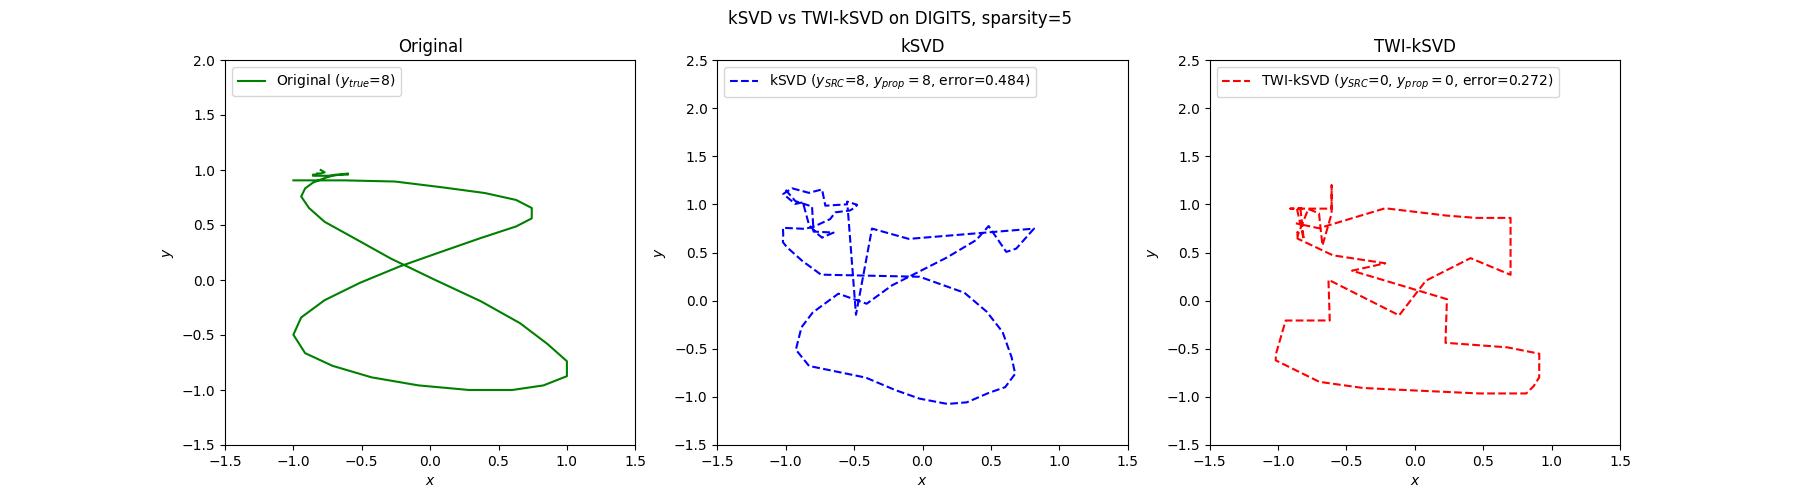
\includegraphics[width=\textwidth]{../../figures/2D_example_sparsity_5.png}
        \caption{Sparsity = 5}
    \end{subfigure}

    \begin{subfigure}[t]{\textwidth}
        \centering
        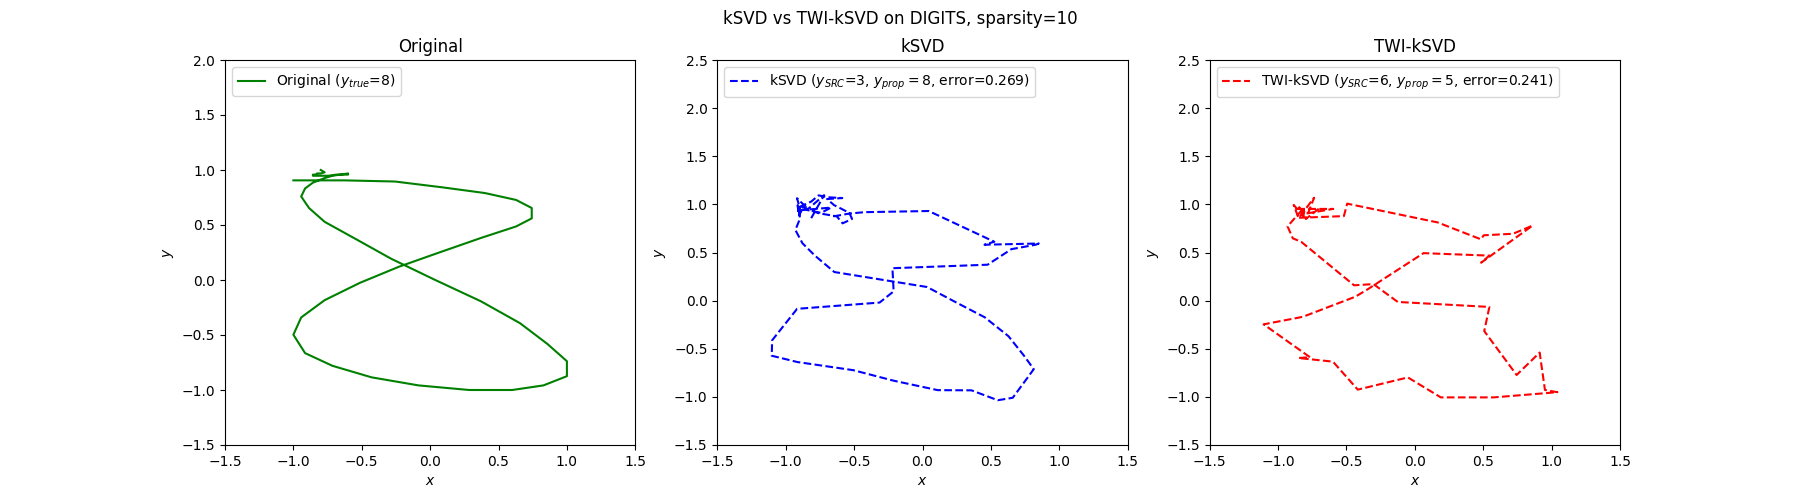
\includegraphics[width=\textwidth]{../../figures/2D_example_sparsity_10.png}
        \caption{Sparsity = 10}
    \end{subfigure}
        \caption{Example of reconstructions (DIGITS dataset) with different sparsity levels}\label{tab:2D_example}
\end{figure*}


{\small
\bibliographystyle{acm}
\bibliography{biblio}
}


\end{document}
